\documentclass{article}

%% PAQUETES

% Paquetes generales
\usepackage[margin=2cm, paperwidth=210mm, paperheight=297mm]{geometry}
\usepackage[spanish]{babel}
\usepackage[utf8]{inputenc}
\usepackage{gensymb}

% Paquetes para estilos
\usepackage{textcomp}
\usepackage{setspace}
\usepackage{colortbl}
\usepackage{color}
\usepackage{color}
\usepackage{upquote}
\usepackage{xcolor}
\usepackage{listings}
\usepackage{caption}
\usepackage[T1]{fontenc}
\usepackage[scaled]{beramono}

% Paquetes extras
\usepackage{amssymb}
\usepackage{float}
\usepackage{graphicx}

%% Fin PAQUETES


% Definición de preferencias para la impresión de código fuente.
%% Colores
\definecolor{gray99}{gray}{.99}
\definecolor{gray95}{gray}{.95}
\definecolor{gray75}{gray}{.75}
\definecolor{gray50}{gray}{.50}
\definecolor{keywords_blue}{rgb}{0.13,0.13,1}
\definecolor{comments_green}{rgb}{0,0.5,0}
\definecolor{strings_red}{rgb}{0.9,0,0}

%% Caja de código
\DeclareCaptionFont{white}{\color{white}}
\DeclareCaptionFont{style_labelfont}{\color{black}\textbf}
\DeclareCaptionFont{style_textfont}{\it\color{black}}
\DeclareCaptionFormat{listing}{\colorbox{gray95}{\parbox{16.78cm}{#1#2#3}}}
\captionsetup[lstlisting]{format=listing,labelfont=style_labelfont,textfont=style_textfont}

\lstset{
	aboveskip = {1.5\baselineskip},
	backgroundcolor = \color{gray99},
	basicstyle = \ttfamily\footnotesize,
	breakatwhitespace = true,   
	breaklines = true,
	captionpos = t,
	columns = fixed,
	commentstyle = \color{comments_green},
	escapeinside = {\%*}{*)}, 
	extendedchars = true,
	frame = lines,
	keywordstyle = \color{keywords_blue}\bfseries,
	language = Oz,                       
	numbers = left,
	numbersep = 5pt,
	numberstyle = \tiny\ttfamily\color{gray50},
	prebreak = \raisebox{0ex}[0ex][0ex]{\ensuremath{\hookleftarrow}},
	rulecolor = \color{gray75},
	showspaces = false,
	showstringspaces = false, 
	showtabs = false,
	stepnumber = 1,
	stringstyle = \color{strings_red},                                    
	tabsize = 2,
	title = \null, % Default value: title=\lstname
	upquote = true,                  
}

%% FIGURAS
\captionsetup[figure]{labelfont=bf,textfont=it}
%% TABLAS
\captionsetup[table]{labelfont=bf,textfont=it}

% COMANDOS

%% Titulo de las cajas de código
\renewcommand{\lstlistingname}{Código}
%% Titulo de las figuras
\renewcommand{\figurename}{Figura}
%% Titulo de las tablas
\renewcommand{\tablename}{Tabla}
%% Referencia a los códigos
\newcommand{\refcode}[1]{\textit{Código \ref{#1}}}
%% Referencia a las imagenes
\newcommand{\refimage}[1]{\textit{Imagen \ref{#1}}}


\begin{document}

% Inserción del título, autores y fecha.
\title{\Large 75.42 Taller de Programación I \\ 
	  \medskip\Huge Informe: Ejercicio N° 1  \\
	  \bigskip\Large\textit{``Cálculo de Multas Eléctricas''}}
\date{}
\maketitle




% INTRODUCCIÓN
\section{Introducción}

	A causa de los múltiples apagones ocurridos en los últimos días, el ENRE (Ente Nacional Regulador Eléctrico) se nos ha solicitado un programa que permita, dado un archivo que almacena un listado de interrupciones de servicio, calcular las multas a aplicar a las distribuidoras de servicio eléctrico. Las multas están basadas en la frecuencia y duración de las mismas, así como en el consumo típico de los clientes.
	\par
	Detalles mas precisos de la problemática y de las condiciones preestablecidas se pueden encontrar en el enunciado del ejercicio\footnote{Se ha evitado hacer un relevamiento de la totalidad de la información que nos fue conferida, de manera de poder mantener el foco del informe en la forma en que se ha encarado la solución del problema}.
\bigskip




% CONSIDERACIONES DE DISEÑO
\section{Consideraciones de diseño}

	Para la correcta implementación de la solución fue necesario plantear y establecer cómo se debería comportar el sistema ante ciertas situaciones que no fueron especificadas en el enunciado del problema. A continuación se listan las contemplaciones instauradas:

\begin{itemize}
	\itemsep=3pt \topsep=0pt \partopsep=0pt \parskip=0pt \parsep=0pt

	\item En caso de no poder ser abierto el archivo, se lanzará un mensaje de error a la salida estándar, y el programa retornará 0;

	\item Se considera que los parámetros recibidos por el ejecutable son del tipo esperado (los primeros cuatro serán enteros, correspondientes a los valores \textit{x\_m}, \textit{x\_f}, \textit{x\_d} y \textit{x\_p}, y el quinto será el \textit{nombre del archivo}, incluyendo su extensión);

	\item En caso de ingresar un archivo vacío, no se enviará resultado ni error alguno a través de la salida estándar, sino que simplemente se finalizará la ejecución retornando 0.

	\item Se supone que, en caso de contener datos el archivo de interrupciones, estos se encontrarán estrictamente dispuestos con el formato \textit{(número\_cliente):(consumo\_típico):(duración\_interrupción)}, dejando en el usuario la responsable de asegurar el cumplimiento de este;

	\item En caso de producirse la superación de tolerancias al mismo tiempo (tolerancia de interrupción por frecuencia y tolerancia de interrupciones por duración acumulada), se realizará el cálculo de la multa tomando en cuenta la tolerancia de interrupción por frecuencia. Dicha elección se tomó considerando que se debe cobrar la multa mas cara entre las posibles.

\end{itemize}
\smallskip




% DISEÑO
\section{Diseño}

	Como creemos que la escalabilidad de un sistema (en este caso del programa) es muy importante, es que se ha decidido modularizar consistentemente ciertas partes que conforman las especificaciones, de manera de permitirnos, en un futuro, agregar o mejorar más fácilmente el funcionamiento del mismo. Es así que, se han dispuesto los filtros de interrupciones y las tolerancias en archivos separados. Esto brinda además un código más ordenado, limpio, legible y mantenible.
	\par
	En los apartados que siguen pondremos la atención en aquellos aspectos de la implementación que pueden ser relevantes a causa de su complejidad o particularidad. En estos se describen los inconvenientes que presentan y la forma en que fueron resueltos.
\bigskip


% DISEÑO - Procesamiento de interrupciones por cliente
\subsection{Procesamiento de interrupciones por cliente}

	Ciertamente, la mayor complejidad de este problema es lograr procesar el archivo evitando la carga total de datos en memoria. Es decir, se busca leer línea por línea (en cada una de ellas se registra una interrupción ligada a cierto cliente) e ir procesándolas. El inconveniente surge cuando notamos la necesidad de considerar todas las interrupciones relacionadas a un mismo proveedor, con el fin de llevar a cabo el cálculo del monto de la multa a aplicar a este último. 
	\par
	Como solución, se optó por utilizar una variable auxiliar que nos servirá de patrón de comparación en cada iteración sobre las líneas. Esta variable es inicializada en 0, simbolizando así que no ha sido sensada aún ninguna interrupción. Al procesar la primer interrupción, la variable tomará el valor del número de cliente correspondiente a esta. De esta manera, en cada procesamiento de línea, se comparará el cliente correspondiente a dicho registro con la variable patrón. Esto nos lleva a que, de mantenerse iguales, estaremos en presencia de interrupciones ligadas a un mismo cliente. 
	\par
	Ahora, si la comparación da como resultado una desigualdad de números de cliente, se nos estará indicando el fin del registro de interrupciones de un proveedor, y el inicio de otro conjunto de datos pertenecientes a otro prestador de servicio eléctrico. Es en este momento cuando se procede a calcular la multa para el proveedor anterior, enviándose los resultados a la salida estándar. Luego, la variable patrón actualiza su valor, almacenando ahora la del cliente mas reciente y volviendo a repetirse todo el proceso nuevamente hasta no poder iterar más, señal de que se ha llegado al fin del archivo.
	\par
	Puesto que nuestra lógica de diseño nos lleva a calcular la multa del cliente anterior respecto del cual nos encontramos posicionados al momento de que ha cambiado el proveedor de servicios, ocurre que, finalizada la iteración, nos faltará calcular la multa correspondiente a las interrupciones del último cliente registrado en el archivo. Por esta razón, al finalizar la iteración sobre las líneas, se procede a calcular la multa del último cliente, lo cual se invoca fuera del bucle. Cabe notar que, para cumplir con las consideraciones de diseño, este último paso es salteado en aquellas circunstancias en las que el archivo se encuentre vacío, siendo detectable esto al corroborar si la variable patrón a modificado su valor inicial nulo.
	\par
	La solución aquí expuesta puede ser visualizada más claramente en el diagrama de flujo mostrado en la \textit{Sección 4}.
	\bigskip



% DISEÑO - Alternativa a función strtok()
\subsection{Alternativa a función \textit{strtok()}}

	Al analizar una línea de registro de interrupción, lo primero que debemos hacer es obtener la información que en ella se encuentra almacenada con el formato \textit{(número\_cliente):(consumo\_típico):(duración\_interrupción)}. En primera instancia, recurrimos a utilizar la función de la libreria string.h, \textit{strtok()}, la cual nos permite separar strings de acuerdo a un patrón especificado. Desafortunadamente, dicha función no soporta operaciones multihilo de forma segura, razón por la cual se recomienda evitar su utilización. Una opción sugerida es la útilización de la función \textit{strtok\_r()}, pero, para nuestra desgracia, dicha función no es parte del estándar C99 al cual nos encontramos sujetos.
	\par
	Por lo tanto, se optó por codificar funciones artesanales que se encarguen, dada una línea del archivo, de devolver el número de cliente, el consumo típico o la duración de la interrupción correspondiente. Estas funciones fueron definidas como: \textit{obtener\_cliente()}, \textit{obtener\_consumo\_tipico()} y \textit{obtener\_duracion\_interrupcion()}. En ellas se utiliza la función \textit{strstr()}, la cual nos devuelve el string original truncado hasta la primer aparición del patrón deseado. Por ejemplo, si se procesa el string \textit{``3236:32:5''} con la función, esta devolverá la cadena \textit{``:32:5''}. Considerando esta última, podemos obtener su longitud, que para nuestro ejemplo es 5. De esta manera, si restamos dicha longitud a la longitud del string original, tendremos la longitud de la cadena que aparece antes del patrón. Finalmente, utilizando la función \textit{strncpy()}, podemos copiar los primeros \textit{n} caracteres del string, siendo justamente \textit{n} la longitud recien obtenida.
	\par
	Para obtener los sucesivos valores de la cadena, simplemente se elimina el patrón ``:'' de la cadena devuelta por la función \textit{strstr()}, lo cual se logra utilizando el operador \textit{``++''} antepuesto a la cadena, y se vuelve a repetir desde este punto el proceso inicial.
	\bigskip\smallskip




% ESQUEMA DEL DISEÑO
\section{Esquema del diseño}

	A continuación, en la \textit{Figura 1}, se muestra el diagrama de flujo que representa la solución implementada del problema presentado. 

\newpage
% Figura 1
\begin{figure}[h]
	\centering
	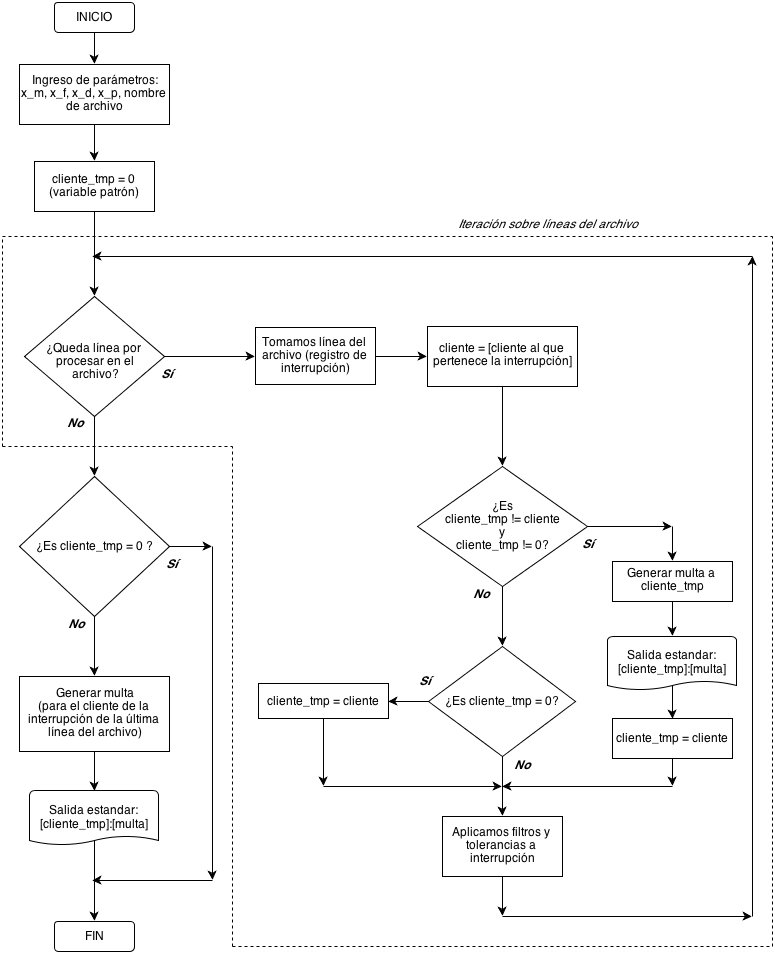
\includegraphics[width=0.91\textwidth]{images/diagrama01.png}
	\medskip
	\caption{Diagrama de flujo representativo de la solución.}
\end{figure}
\bigskip\bigskip
	

\end{document}
